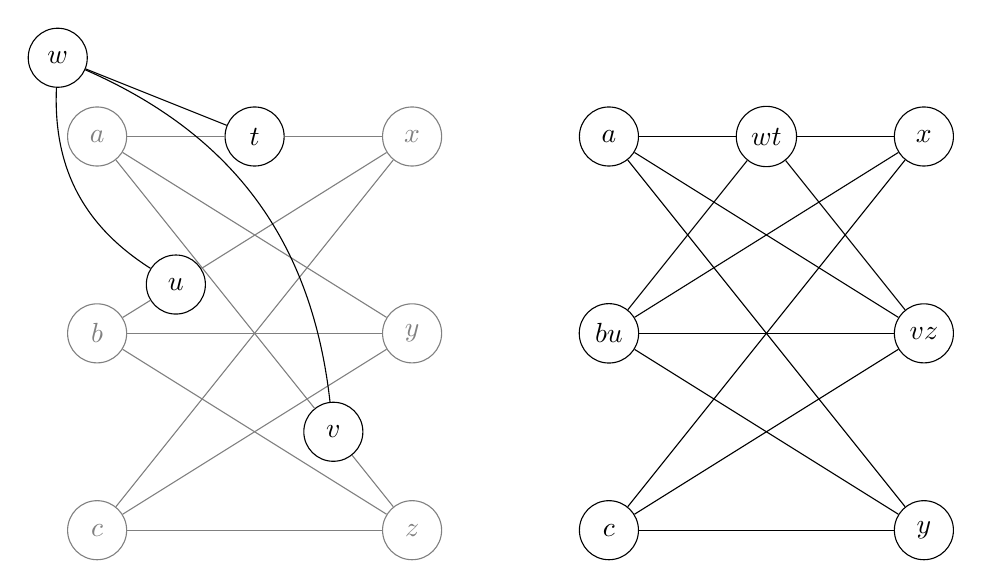
\begin{tikzpicture}
\node [circle, minimum height=0.75cm, color=gray, draw] (a) at (0,0) {$a$};
\node [circle, minimum height=0.75cm, color=gray, draw] (b) at (0,-2.5) {$b$};
\node [circle, minimum height=0.75cm, color=gray, draw] (c) at (0,-5) {$c$};
\node [circle, minimum height=0.75cm, color=gray, draw] (x) at (4,0) {$x$};
\node [circle, minimum height=0.75cm, color=gray, draw] (y) at (4,-2.5) {$y$};
\node [circle, minimum height=0.75cm, color=gray, draw] (z) at (4,-5) {$z$};

\node [circle, minimum height=0.75cm, draw] (t) at (2,0) {$t$};
\node [circle, minimum height=0.75cm, draw] (u) at (1,-1.88) {$u$};
\node [circle, minimum height=0.75cm, draw] (v) at (3,-3.75) {$v$};
\node [circle, minimum height=0.75cm, draw] (w) at (-0.5,1) {$w$};

\draw [color=gray] (a) edge (t);
\draw [color=gray] (t) edge (x);
\draw [color=gray] (a) edge (y);
\draw [color=gray] (a) edge (v);
\draw [color=gray] (v) edge (z);
\draw [color=gray] (b) edge (u);
\draw [color=gray] (u) edge (x);
\draw [color=gray] (b) edge (y);
\draw [color=gray] (b) edge (z);
\draw [color=gray] (c) edge (x);
\draw [color=gray] (c) edge (y);
\draw [color=gray] (c) edge (z);

\draw  (w) edge (t);
\draw [bend right] (w) edge (u);
\draw [bend left] (w) edge (v);

\node [circle, minimum height=0.75cm, draw] (v1) at (6.5,0) {$a$};
\node [circle, minimum height=0.75cm, draw] (v6) at (6.5,-2.5) {$bu$};
\node [circle, minimum height=0.75cm, draw] (v7) at (6.5,-5) {$c$};
\node [circle, minimum height=0.75cm, draw] (v2) at (8.5,0) {$wt$};
\node [circle, minimum height=0.75cm, draw] (v3) at (10.5,0) {$x$};
\node [circle, minimum height=0.75cm, draw] (v4) at (10.5,-2.5) {$vz$};
\node [circle, minimum height=0.75cm, draw] (v5) at (10.5,-5) {$y$};
\draw  (v1) edge (v2);
\draw  (v2) edge (v3);
\draw  (v1) edge (v4);
\draw  (v1) edge (v5);
\draw  (v6) edge (v3);
\draw  (v6) edge (v4);
\draw  (v6) edge (v5);
\draw  (v7) edge (v3);
\draw  (v7) edge (v4);
\draw  (v7) edge (v5);
\draw  (v2) edge (v6);
\draw  (v2) edge (v4);
\end{tikzpicture}